%!TEX root = ../main.tex
%Adding the above line, with the name of your base .tex file (in this case "thesis.tex") will allow you to compile the whole thesis even when working inside one of the chapter tex files
%%
%%
%%%%%%%%%%%%%%%%%%%%%%%%%%%%%%%%%%%%%%%%%%%%%%%%%%%%%%%%%%%%%%%%%%%%%%%%%%%%%
%%%%%%%%%%%%%%%%%%%%%%%%%%%%%%%%%%%%%%%%%%%%%%%%%%%%%%%%%%%%%%%%%%%%%%%%%%%%%
%%%%%%%%%%%%%%%%%%%%%%%%%%%%%%%%%%%%%%%%%%%%%%%%%%%%%%%%%%%%%%%%%%%%%%%%%%%%%
%										FUTURE WORK
%%%%%%%%%%%%%%%%%%%%%%%%%%%%%%%%%%%%%%%%%%%%%%%%%%%%%%%%%%%%%%%%%%%%%%%%%%%%%
%%%%%%%%%%%%%%%%%%%%%%%%%%%%%%%%%%%%%%%%%%%%%%%%%%%%%%%%%%%%%%%%%%%%%%%%%%%%%
%%%%%%%%%%%%%%%%%%%%%%%%%%%%%%%%%%%%%%%%%%%%%%%%%%%%%%%%%%%%%%%%%%%%%%%%%%%%%
\onehalfspacing
\chapter{Future Work}
\label{chap:future}
%The future work of this PhD will be twofold combining the technical tasks required to get REALTA and TACl working to their full potential, 
The future work of this PhD can be divided into 3 main topics; technical work with REALTA and TACl, analysis of fine spatial structure in a complex radio burst, and radio frequency interference (RFI) removal using machine learning. A Gantt chart for the remainder of this PhD is shown in Figure \ref{fig:Gantt}

\begin{figure}[t]
    \centering
    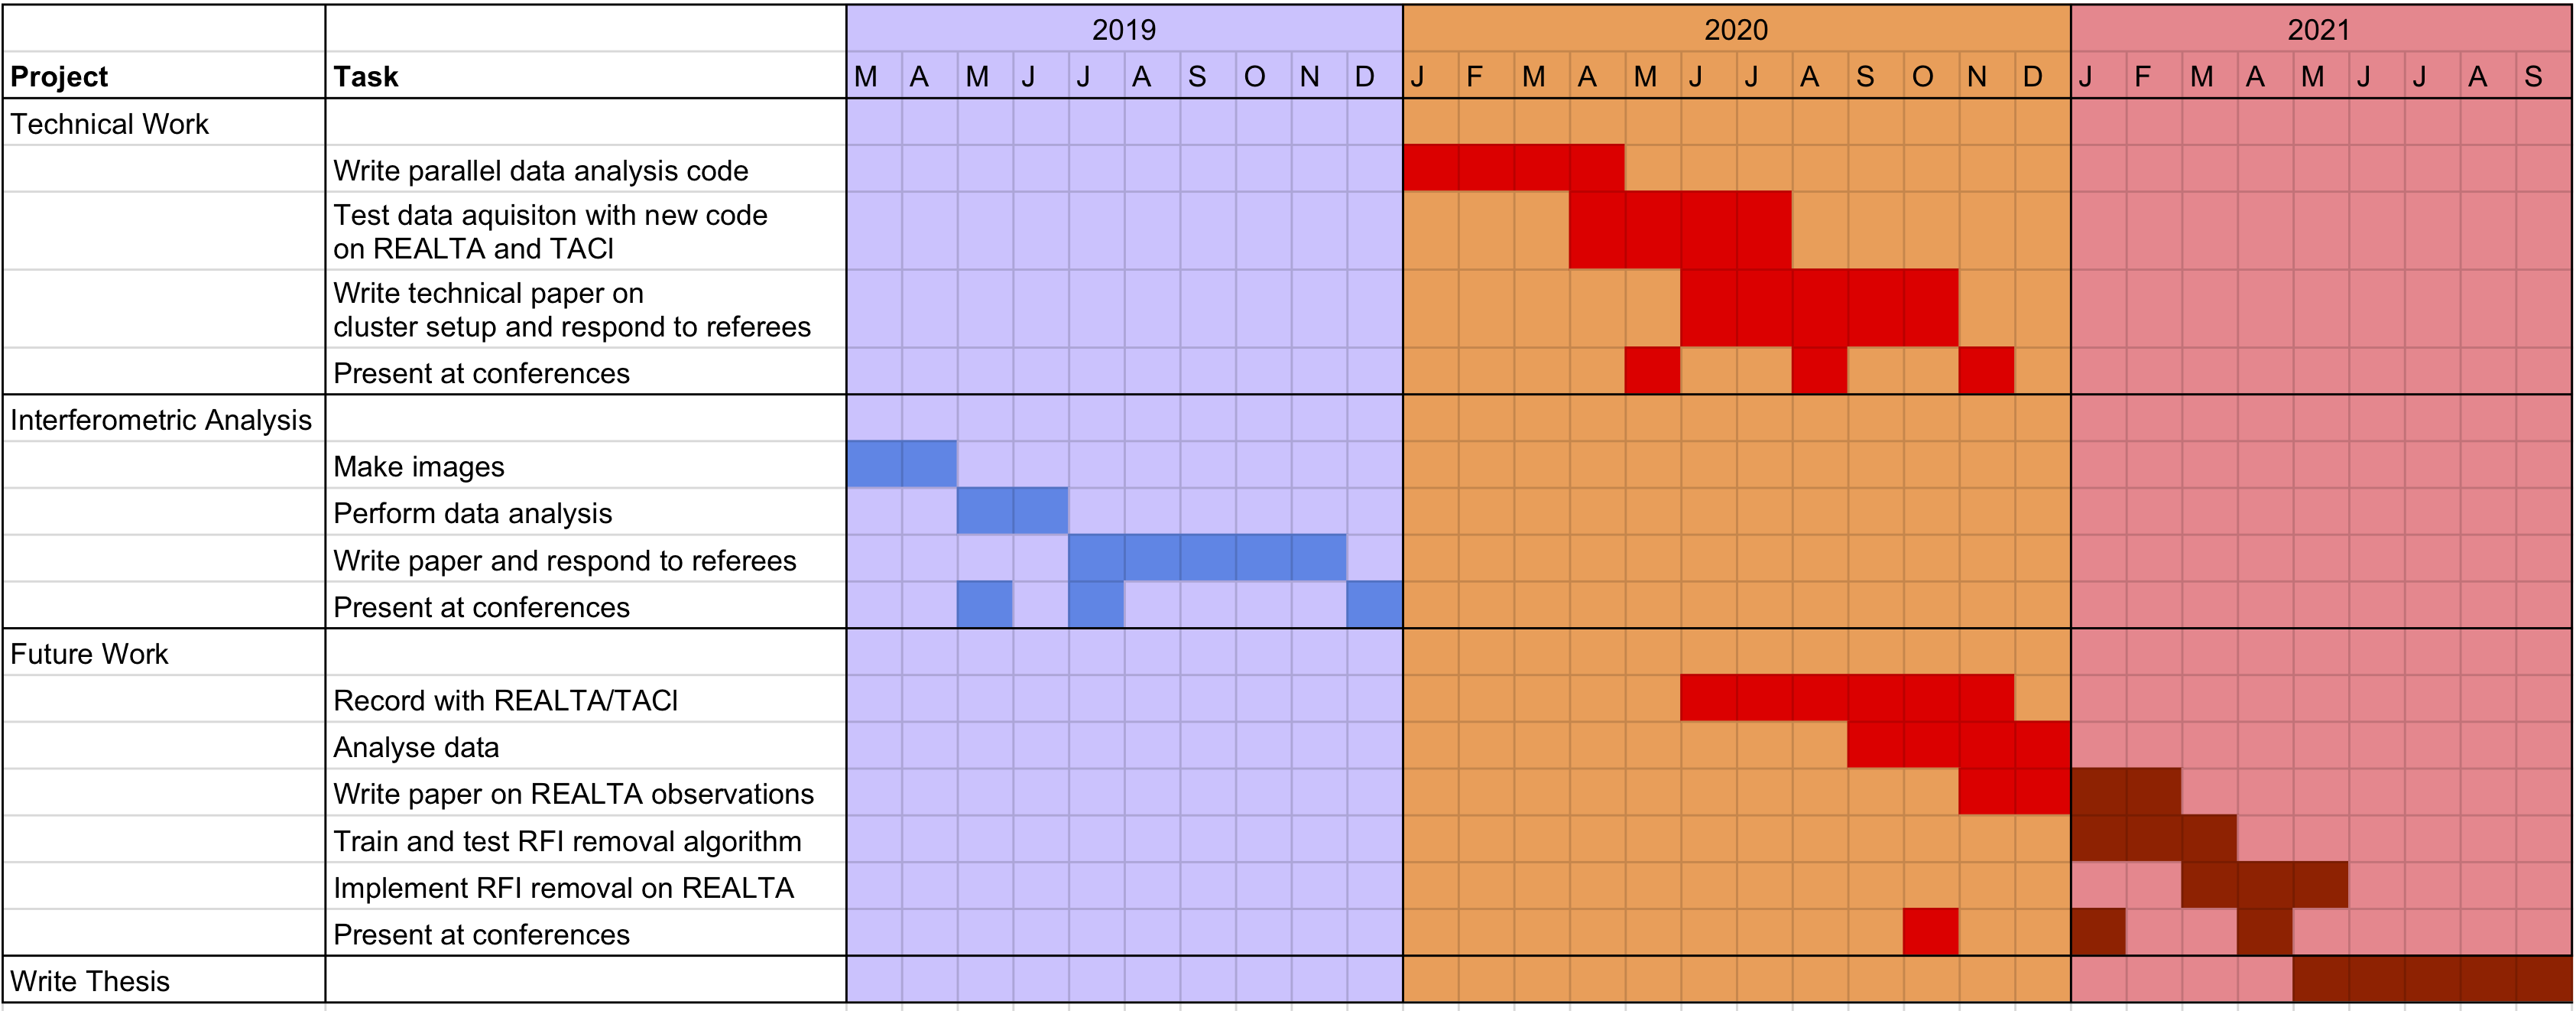
\includegraphics[width=0.75\columnwidth]{Images/PM_Ganttchart.png}
    \caption[Gantt chart for remainder of PhD]{Gantt chart for remainder of PhD}
    \label{fig:Gantt}
\end{figure}

\section{Technical Work}
Both REALTA and TACl are operational in a minimal sense although there is still work to be done in order to develop them to become bona fide telescope backends. Data recorded by TACl in the last number of months has been partially corrupted and the cause is still being investigated with Dr. Brian Coghlan of the School of Computer Science and Statistics. Once operational, TACl will be able to record TBB data again and the development of software to analyse this data will be continued. Despite being in solar minimum, approximately 2,355 radio bursts are expected to occur per year \citep{Nita2002}. This give ample opportunity to detect a radio burst and study it at the highest temporal resolution ever. %It is expected that some sort of solar radio phenomenon will be detected by the TBBs and analysed before the end of this PhD.

REALTA also requires further setup before it can be used as a parallel GPU-based cluster. A head node to control the cluster operations was installed in November 2018 and collaboration with Griffin Foster (Oxford, Berkeley, Breakthrough) will continue in order to write GPU-based code for data capture and analysis. This will make observations of the Sun more accessible than they are currently which should result in greater scientific output.

After REALTA is capable of performing analysis on incoming data in real time a paper discussing the hardware and software setup required to do so could be written. This would be the first of its kind for an international LOFAR station and would hopefully inspire other international station owners to improve their own computing hardware. This would allow the possibility of more computationally intense collaborations with other international stations operating in single station mode.

\section{Interferometric Analysis}
Analysis of the burst event described in section \ref{sec:event} will continue and be presented at an international conference by the end of 2019. It is expected that this analysis will put a limit on how much scattering affects radio propagation in the corona. If it is shown that there is no fundamental limit to spatial resolution at metric limits this will strengthen the case to observe the Sun with the full $\sim 2000$ km international baseline offered by LOFAR.

There are a number of steps that must be carried out before this can be done however, the most immediate of which is to account for the change in coordinate systems from topocentric (from the viewers perspective) to heliocentric (centred on the Sun). This will allow close comparison of radio and other wavelength observations, e.g. EUV data from AIA, as this is the standard coordinate system used in solar physics.
The imaging of this event must also be thoroughly investigated as a change in the parameters used in the WSCLEAN algorithm can result in drastically different images. As such, weighting schemes, number of iterations and more must be considered with great thought before data analysis of images can begin.
Once images have been created, the spatial scale and distance from the centre of the Sun will be measured in order to obtain a measure on how much propagation effects in the corona effect the measurement.

The existence of striae in the Type III spectrum offer a direct comparison with the work by \cite{Kontar2017} using interferometric imaging for the first time. It is expected that this work will be submitted as a letter at a well renowned journal such as the Astrophysical Journal.

\section{RFI Removal}
Radio Frequency Interference often obscures signals of interest in dynamic spectra and usually washes out weaker signals because it is so intense. Great effort is made in the design of radio telescopes to mitigate the effects of nearby electronics however to eliminate all RFI completely would require such a massive societal involvement that it will never happen. Thus, removal of RFI is done after data has been recorded using algorithms developed to identify RFI based on its spectral properties \citep{Offringa2012b, Nita2007}.

Machine learning techniques can be used to detect and remove RFI without the need to define an algorithm based on RFI structure. An approach to removing RFI is inspired by a transient detection system described by \cite{Sedaghat2018}. A convolutional autoencoder (CAE) is a machine learning algorithm using convolutional layers in a traditional autoencoder \citep{Vincent2008}. A CAE would be used to first encode a spectrum containing RFI to a more simple form and then decode to return the spectrum without RFI. This procedure is known as ``denoising" and has seen success in a number of classical machine learning problems. To train the network successfully will require many hundereds of thousands of sample spectra. One hundred thousand LOFAR LBA spectra have been simulated, these will be used as a first attempt training set for the CAE and its performance will be tested on 20\% of these spectra. It is anticipated to test this network on real I-LOFAR data in conjuction with an automatic burst detection network developed by Dr. Eoin Carley of the Solar and Space Weather group.


%Currently this project is in its early stage but is outlined as follows. 100000 LOFAR spectra are simulated with and without RFI. These spectra will be fed into what is known as a convolutional encoder-decoder network or convolutional autoencoder (CAE) which will learn how to remove RFI without the need for a pre-made algorithm based on the physics of RFI, such as spectral kurtosis RFI removal described by \cite{Nita2007}. CAEs are based on the principals of autoencoders described in \cite{Vincent2008} but using the convolutional methods that have seen great success in image processing.
